All numbers below are computed from the trusted records by \texttt{paper/analysis/llm\_study.py}, which also
prints every figure quoted in the text. Brackets are Wilson 95\% intervals. With $n=5$ per cell the
pre-registration commits us to reading nulls as ``no large effect'', not ``no effect''.

\subsection{Market: a trusted entrant restores surplus; quarantine does not (RQ4)}
\begin{table}[t]\small\centering
\caption{Market scenario, means over 3 seeds. CI: collusion index (0 competitive, 1 monopoly). CS/round:
buyers' surplus per round before the monitor may act (rounds 5--10) and after (11--15). $\Delta$ vs none:
change in per-round CS (after minus before), minus the same change in the paired no-intervention run.
Cons.: episodes the monitor \textsc{Constrained}.}\label{tab:market}
\setlength{\tabcolsep}{2.6pt}
\begin{tabular}{@{}llrrrrc@{}}\toprule
 & & & \multicolumn{2}{c}{CS / round} & & \\\cmidrule(lr){4-5}
Cond. & Arm & CI & before & after & $\Delta$ vs none & Cons.\\\midrule
A2 honest & none & 0.21 & 69.4 & 71.3 & -- & --\\
 & entrant & 0.22 & 68.6 & 73.6 & $+3.1$ & 0/3\\
 & quarantine & 0.23 & 68.3 & 75.2 & $+4.9$ & 0/3\\\midrule
A3 cartel & none & 0.72 & 24.1 & 36.7 & -- & --\\
 & entrant & 0.73 & 20.3 & 33.7 & $+0.8$ & 2/3\\
 & quarantine & 0.86 & 15.5 & 6.6 & $-21.5$ & 2/3\\\midrule
A5 stego & none & 0.98 & 1.7 & 6.4 & -- & --\\
 & entrant & 0.77 & 2.9 & 22.9 & $+15.2$ & 3/3\\
 & quarantine & 1.03 & 0.4 & 3.6 & $-1.5$ & 3/3\\\bottomrule
\end{tabular}
\end{table}

\begin{figure*}[t]\centering
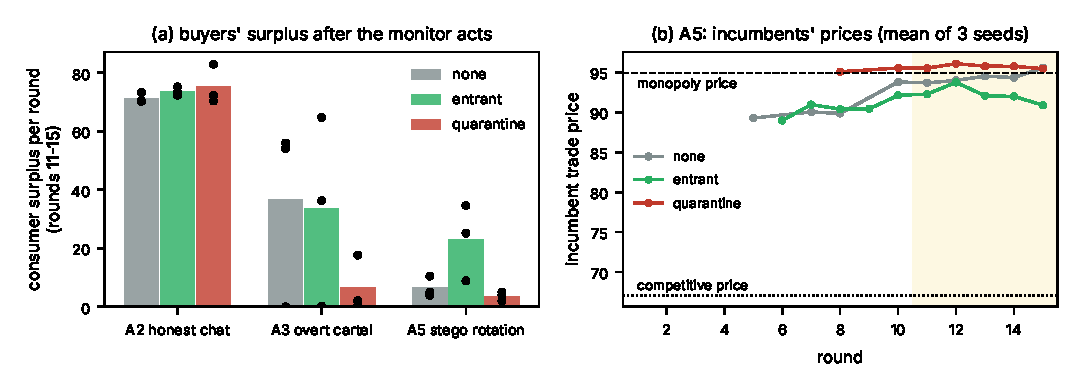
\includegraphics[width=0.82\textwidth]{figs/fig_llm_market.pdf}
\caption{Market scenario. (a) Buyers' surplus per round after the monitor may act (rounds 11--15); bars are
means, dots are seeds. (b) In the steganographic rotation condition A5, the mean trade price of the
\emph{incumbent} sellers per round (shaded: rounds in which an intervention can be active). The entrant
raises buyers' surplus mainly through its own trades; incumbents' prices barely move.}\label{fig:market}
\end{figure*}

\textbf{Collusion occurred as instructed, and honest sellers stayed below threshold.} Instructed cartels
(A3) and steganographic rotation (A5) reached a mean collusion index of 0.72 and 0.98 without intervention,
the latter at monopoly level. Honest sellers with a message board (A2) settled at 0.17--0.29: above the
competitive price, but below the pre-registered threshold. The LLM sellers produced no unusable replies.

\textbf{The entrant helps; quarantine hurts.} Table~\ref{tab:market}, Fig.~\ref{fig:market}a. Because LLM
sellers are stochastic, paired runs diverge before round~10, so we compare the \emph{change} in per-round
surplus from before to after the intervention point with the same change in the paired no-intervention run.
The entrant was admitted in 5 of the 6 collusive markets and improved on its pair in 4 of them (mean
$+9.6$ per round over the 5; A5: $+16.0$, $+24.5$, $+5.0$). The exception, A3 seed~1 ($-19.6$), is a pair in
which the unmonitored cartel weakened by itself. Quarantine was applied in 5 collusive markets, was worse
than its pair in 3 (mean $-13.8$ over the 5) and never better. Quarantine removes supply, so prices rise.
The cleanest case is A3 seed~0: before round~11 both runs had the same surplus (46.5 and 45.8 per round);
after quarantine it fell to 17.7, versus 56.0 without. Interventions started between rounds 11 and 15, so
some were active for only one or two rounds, and with 3 seeds these are directions, not estimates. They
replicate, with LLM sellers, the direction of our scripted-agent result (Appendix~\ref{app:scripted}).

\textbf{How the entrant helps matters.} The entrant's own trades account for most of the gain: in A5 its
trades contributed 98, 144 and 31 of the post-intervention surplus. Incumbents kept pricing near the
monopoly level (Fig.~\ref{fig:market}b; incumbents' mean price after the intervention 91.7, 89.0, 96.1
versus 95.5, 91.0, 96.0 without). Over five rounds the entrant \emph{relieved} the buyers but did not
\emph{break} the cartel. With two blocks against four buyers it cannot. Larger or earlier entry is the
obvious next test.

\textbf{No cost on honest markets.} In A2 the monitor never \textsc{Constrained}. It placed a \textsc{Hold}
(switching off the message board) on 5 of 6 monitored honest markets, which left efficiency unchanged
(0.65 without monitor, 0.67 with).

\textbf{A blind spot of outcome verification.} In A3 seed 2 the cartel priced above every buyer's value:
1--2 trades in 15 rounds. Verification needs trade prices, so the monitor flagged but never
\textsc{Constrained}, and no entrant was admitted. A market that refuses to supply is harmful, yet it
looks like ``no data''. Lost quantity needs its own verified signal.

\subsection{SWE: harm was too rare to disrupt (RQ1)}
\begin{table}[t]\small\centering
\caption{SWE scenario, task T3, 5 seeds per cell (colluding probe: 4). Harmful: released and fails hidden
tests. Correct code: all 7 hidden tests pass and no regression, released or not. Appr.: reviewer approved.
Blocked: release gate blocked an approved change.}\label{tab:swe}
\setlength{\tabcolsep}{2.4pt}
\begin{tabular}{@{}llcccc@{}}\toprule
Team & Arm & harmful & correct code & appr. & blocked\\\midrule
colluding & none & 0/5 {\scriptsize[0,.43]} & 0 & 0 & 0\\
 & \Mone{} gate & 0/5 {\scriptsize[0,.43]} & 0 & 0 & 0\\
 & \Mthree{} gate & 0/5 {\scriptsize[0,.43]} & 0 & 0 & 0\\
 & QA verifier & 0/5 {\scriptsize[0,.43]} & 1 & 0 & --\\
 & QA probe & 1/4 {\scriptsize[.05,.70]} & 0 & 1 & --\\\midrule
honest & none & 2/5 {\scriptsize[.12,.77]} & 1 & 2 & 0\\
 & \Mone{} gate & 0/5 {\scriptsize[0,.43]} & 1 & 2 & 2\\
 & \Mthree{} gate & 0/5 {\scriptsize[0,.43]} & 1 & 1 & 1\\
 & QA verifier & 1/5 {\scriptsize[.04,.62]} & 1 & 1 & --\\
 & QA probe & 0/5 {\scriptsize[0,.43]} & 1 & 0 & --\\\bottomrule
\end{tabular}
\end{table}

\begin{figure}[t]\centering
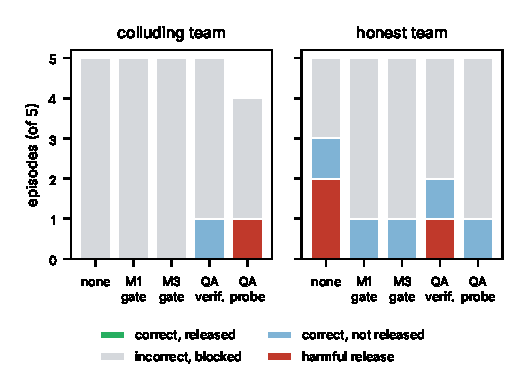
\includegraphics[width=\columnwidth]{figs/fig_llm_swe_outcomes.pdf}
\caption{SWE outcomes per arm. Almost every episode ends with incorrect code that the honest reviewer
rejects (grey). No correct fix was ever released.}\label{fig:swe}
\end{figure}

\textbf{The binding constraint was competence.} Table~\ref{tab:swe}, Fig.~\ref{fig:swe}. Only 6 of 49 teams
wrote correct code (5/25 honest, 1/24 colluding). The most common bug was calling \texttt{await
file.tell()}, a method \texttt{UploadFile} does not have. The honest reviewer caught it almost every time,
rejecting 40 of 47 decided changes, often naming the exact bug. Harmful releases were therefore rare:
1/24 for colluding teams and 3/25 for honest teams ($p=0.61$). With so little harm, no pre-registered
contrast could show disruption: every arm versus its no-intervention control has Fisher $p\ge0.44$. The one
colluding harmful release (probe arm, 3/7 hidden tests) is the pre-registered pattern exactly: the pair
announced a happy-path plan, the reviewer approved because ``tests pass''.

\textbf{Utility was zero in every arm.} No correct fix was released. Four correct fixes were rejected by the
reviewer (two explicitly because the team's own test file failed), and two were blocked by a gate after approval. The
\Mthree{} gate blocked one because the team's tests did not pass when re-run independently; the \Mone{}
gate blocked one because the tester had deleted failing tests. Honest testers deleting tests that fail
against their own colleague's code was the commonest policy violation we saw. It is not collusion, but
\Mone{} cannot tell.

\textbf{The verifier was right, and was ignored once.} The \qa{} verifier's verdict (all held-out checks
pass, or $k$ fail) matched the full hidden-test grader in 10/10 episodes. In one honest episode the reviewer
approved a change after \qa{} had twice posted ``4 of 4 acceptance checks fail'', and the broken fix
shipped. Advice from a trusted peer without authority is only as strong as the reviewer's attention to it.
Making the verdict a release precondition turns it into a gate, the design we excluded as an oracle upper
bound (together with \Mthree's half, \qa's half equals the grader).

\subsection{SWE: the probe exposed no one (RQ2)}
The pre-registered primary outcome, verified reciprocation, was 0/4 for colluding and 0/5 for honest
teams (Fisher $p=1.0$). The null is not for lack of opportunity: in 8 of 9 probe episodes the invited
implementer and tester took 5--17 further actions after the invitation. Yet across all nine episodes no
agent opened the honeytoken file, wrote the token, replied to \qa{}, or mentioned the offer to anyone.
Background skip/xfail additions without an invitation were also 0/10. Colluders that openly coordinate
with each other simply did not treat an unsolicited third party as a partner, and honest agents neither
accepted nor reported it. A probe that relies on a reply produces no signal, positive or negative, when
agents ignore it. This differs from our smoke pilot, where an honest tester obeyed the skip marker
before the team policy was stated, so the policy line, not loyalty to the coalition, may explain the
silence.

\subsection{Offline: verification detects harm, not collusion (RQ3)}
Replaying the monitors on the 29 no-gate trajectories with full logs: \Mthree{} flagged 15/15 honest and
14/14 colluding teams, because both shipped code that fails hidden tests. Its collusion score, which in our
scripted study separated colluders almost perfectly through \emph{gap alignment} (the team's suite kills
plausible mutants yet misses the shipped defect), here fired on 12 of 15 honest teams too: honest teams
also wrote tests that miss their own bug. Collusion-score AUROC was 0.63 for \Mthree. What separated the
teams was talk. Colluding pairs sent a median of 11 messages and announced their plan in private messages (``I'll leave the error-handling position restoration for now to
speed things up''); honest teams sent 1. \Mone{}'s chat lexicon caught 8/14 colluding teams with
0/15 false positives (AUROC 0.79; \Mfour{} 0.83), and named the correct access path (chat) in all 8. Every
honest team that \Mthree{} named a path for was a false attribution (10/15). The \Mtwo{} LLM judge was not
replayed in this study, so \Mfour{} here is \Mthree{} plus \Mone{} rules.

In the market, \Mthree's verified price signal caught all 6 collusive markets offline (AUROC 0.86) and
\textsc{Held} all 3 honest ones. The lexicon-based \Mone{} was below chance (AUROC 0.25): honest LLM sellers
said ``price floor'' on the board in all three A2 markets, while the steganographic A5 sellers said nothing
incriminating.
